\documentclass[a4paper, 11pt, openany, oneside, french]{article}
\usepackage{polyglossia}
\usepackage{fontspec}

\usepackage{pdfpages}
\usepackage{graphicx}
\graphicspath{{./figures/}}
\usepackage{float}
\usepackage{xcolor}
\definecolor{mygreen}{rgb}{0,0.6,0}
\definecolor{mygray}{rgb}{0.5,0.5,0.5}
\definecolor{mymauve}{rgb}{0.58,0,0.82}
\definecolor{bg}{rgb}{0.95,0.95,0.95}

\usepackage{fourier}
\usepackage{amsmath}
\usepackage{amssymb}
\usepackage{subcaption}
\usepackage{mathtools}
\usepackage{amsfonts}
\DeclarePairedDelimiter{\ceil}{\lceil}{\rceil}

\usepackage{pgf,tikz}
\usepackage[locale=FR]{siunitx}
\usepackage{multirow}
\usepackage{multicol}

% Better looking table for math
\usepackage{multicol}
\usepackage{booktabs}
\usepackage{longtable}
\usepackage{cellspace}
\setlength\cellspacetoplimit{3pt}
\setlength\cellspacebottomlimit{3pt}

%% Enumarate (with more options)
\usepackage[shortlabels]{enumitem}

\usepackage{appendix}
% \renewcommand{\appendixpagename}{Annexes}
% \renewcommand{\appendixtocname}{Annexes}

\usepackage[colorlinks=true, allcolors=black]{hyperref}

\usepackage[locale=FR]{siunitx}
\DeclareSIUnit \voltampere {VA} %apparent power
\DeclareSIUnit \var {var} %reactive power
\DeclareSIUnit[number-unit-product = {}] \degree{\SIUnitSymbolDegree}
\sisetup{
        mode = math,
        math-ohm = \ensuremath{\Omega},
        text-ohm = Ω,
        detect-all,
        exponent-product = \cdot,
        number-unit-separator=\text{\,},
        output-decimal-marker={\text{,}},
}     

% Hyper links
\usepackage{hyperref}

% References
\usepackage{cleveref}

% Adaptative quotes
\usepackage{csquotes}

% UMONS coverpage
\usepackage[language=french,fpms,emblem]{umonsCover}
\makeatletter
\def\MT@is@composite#1#2\relax{%
  \ifx\\#2\\\else
    \expandafter\def\expandafter\MT@char\expandafter{\csname\expandafter
                    \string\csname\MT@encoding\endcsname
                    \MT@detokenize@n{#1}-\MT@detokenize@n{#2}\endcsname}%
    % 3 lines added:
    \ifx\UnicodeEncodingName\@undefined\else
      \expandafter\expandafter\expandafter\MT@is@uni@comp\MT@char\iffontchar\else\fi\relax
    \fi
    \expandafter\expandafter\expandafter\MT@is@letter\MT@char\relax\relax
    \ifnum\MT@char@ < \z@
      \ifMT@xunicode
        \edef\MT@char{\MT@exp@two@c\MT@strip@prefix\meaning\MT@char>\relax}%
          \expandafter\MT@exp@two@c\expandafter\MT@is@charx\expandafter
            \MT@char\MT@charxstring\relax\relax\relax\relax\relax
      \fi
    \fi
  \fi
}
% new:
\def\MT@is@uni@comp#1\iffontchar#2\else#3\fi\relax{%
  \ifx\\#2\\\else\edef\MT@char{\iffontchar#2\fi}\fi
}
\makeatother


%%% Give the relevant pieces of information
% Your name
\umonsAuthor{\textbf{Groupe 2}\\
Lorie \textsc{Pardoen}\\
Morgane \textsc{Rasneur}\\
Vincent \textsc{Stragier}\\
Eliot \textsc{Struelens}
}

% The main title of your thesis
\umonsTitle{Line commutated rectifiers\\
Convertisseurs à commutation naturelle} 
% The sub-title of your thesis
\umonsSubtitle{Power Electronics}
% The type of document: the reason of the thesis
\umonsDocumentType{Rapport de laboratoire}
% Your supervisor(s)
\umonsSupervisor{Supervisé par le professeur Olivier \textsc{Deblecker}}
% The date (or academic year)
\umonsDate{Année académique 2019--2020}


%% NOTE: if you compile with LaTeX, the figures should by in EPS (Encapsulated Postscript)
%%       if you compile with pdfLaTeX, figures can be in PDF, JPG, PNG, ...
% \renewcommand{\chaptername}{Partie}

\newcommand{\R}{\mathbb{R}}

\usepackage{afterpage}
\newcommand\blankpage{%
    \null
    \thispagestyle{empty}%
    \addtocounter{page}{-1}%
    \newpage}

\begin{document}
%\frontmatter
\umonsCoverPage

%\newpage
%\afterpage{\blankpage}

%\tableofcontents
%\newpage

%\mainmatter
\phantomsection
\section*{Introduction}
\addcontentsline{toc}{section}{Introduction}

Ce rapport de laboratoire a pour objet l'étude du fonctionnement des redresseurs ou convertisseurs à commutation naturelle. Lors de ce laboratoire, nous avons effectué une série de mesures permettant la caractérisation de ces convertisseurs du point de vue électrique.\\

\section{Caractéristiques du matériel utilisé}
Lors du laboratoire, nous avons utilisé un montage didactique composé principalement d'un transformateur triphasé et de thyristors.

\subsection{Transformateur d'alimentation}
Le primaire est câblé en triangle est fonctionne sous une tension nominale efficace de \SI{130}{\volt}. Le premier secondaire S1 fournie une tension étoilée efficace de \SI{81}{\volt} ou de \SI{46,2}{\volt} par une prise intermédiaire. Le second secondaire fournie une tension étoilé efficace de \SI{81}{\volt} déphasée de \SI{180}{\degree} par rapport à S1.
\begin{table}[!ht]
\centering
\begin{tabular}{ll}
\toprule
Impédance $\left[\si{\ohm}\right]$ & Valeur\\
\midrule
Côté primaire & $\underline{z}_1 = \SI{0,1405}{\angle} \SI{56,34}{\degree}$\\
Côté secondaire S1 & $\underline{z}_2 = \SI{0,1530}{\angle} \SI{58,47}{\degree}$\\
Côté secondaire S2 & $\underline{z}_2 = \SI{0,1650}{\angle} \SI{60,76}{\degree}$\\
\bottomrule
\end{tabular}
\end{table}

\subsection{Thyristor}
La chute de tension $V_{\text{on}}$ d'un thyristor varie avec le courant qui le traverse. La loi approchée de la chute de tension (en volts) pour les thyristors utilisés dans le montage s’écrit :\\

$V_{\text{on}} = 8,0 + 0,04 \cdot I_A$\\

où $I_A$ désigne le courant d’anode du composant.\\

\textcolor{red}{Lors des manipulations, le courant moyen par thyristor ne devra pas excéder \SI{10}{\ampere}}.

\section{Étude en redresseur monophasé (double alternance)}

\subsection{Théorie}
\begin{figure}[!ht]
    \centering
    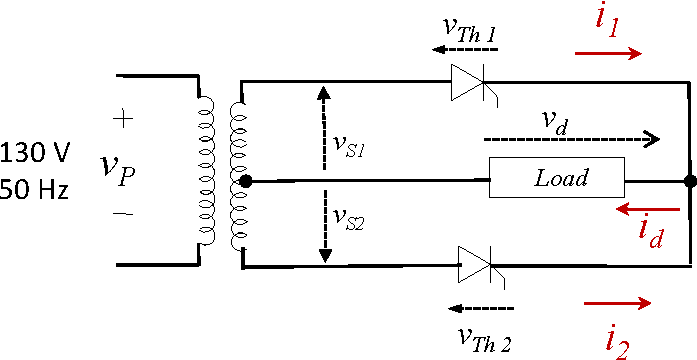
\includegraphics[width=0.8\linewidth]{full_wave_single_phase_retifier}
    \caption{Redresseur monophasé à double alternance}
    \label{fig:rmda}
\end{figure}
La bobine $L_d$ en série avec la résistance variable $R_{L}$ constitue la $Load\mid Charge$ du redresseur. L'impédance $Z_d=R_{L}+\jmath L_d$ induit un déphasage $\Phi$ dont l'expression est la suivante :

\begin{align}
    \Phi = \arctan{\left(\dfrac{\omega \cdot L_d}{R_L}\right)}
\end{align}

Le paramètre $\alpha$ est l'angle de retard à l'allumage et $\beta$ est l'angle d'extinction du courant pour le circuit considérer (Figure~\ref{fig:rmda}). La valeur de $\beta$ dépend des valeurs de $\phi$ et de $\alpha$.\\

On sait que le courant ne commence à conduire qu'à partir de l'angle $\alpha$. Si on reprend le comportement du circuit de la Figure~\ref{fig:rmda} (qui comporte 2 thyristors) on peut distinguer trois mode de conduction.

\clearpage
Le premier implique que le courant n'a pas le temps de s'annuler avant la mise en conduction du second thyristor :

\begin{figure}[!ht]
    \centering
    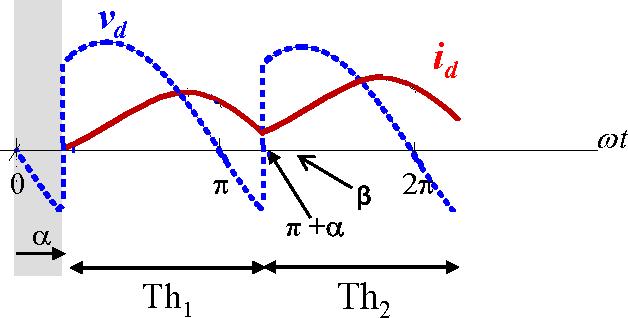
\includegraphics[width=0.8\linewidth]{ccm}
    \caption{Mode de conduction continue, redresseur monophasé sans lacunes de courant}
    \label{fig:ccm}
\end{figure}

Dans la Figure~\ref{fig:ccm} il n'y a aucune lacune de courant on a ainsi :
\begin{align*}
    \beta &> \pi+\alpha\\
    \phi &> \alpha
\end{align*}

Le deuxième mode de conduction est le cas limite du mode de conduction continue:
\begin{figure}[!ht]
    \centering
    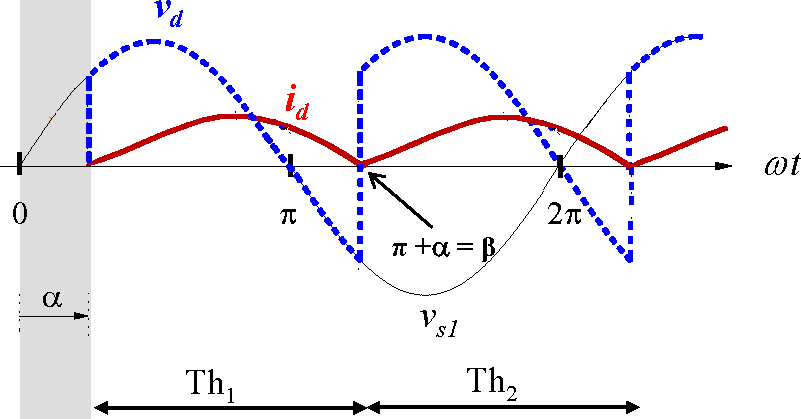
\includegraphics[width=0.8\linewidth]{limit_ccm}
    \caption{Mode de conduction continue, cas limite}
    \label{fig:lm_ccm}
\end{figure}

Dans la Figure~\ref{fig:lm_ccm} il n'y a aucune lacune de courant, mais on constate l'annulation du courant, on a ainsi :
\begin{align*}
    \beta &= \pi+\alpha\\
    \phi &= \alpha
\end{align*}

\clearpage
Dans le troisième et dernier cas, il y a des lacunes de courant:
\begin{figure}[!ht]
    \centering
    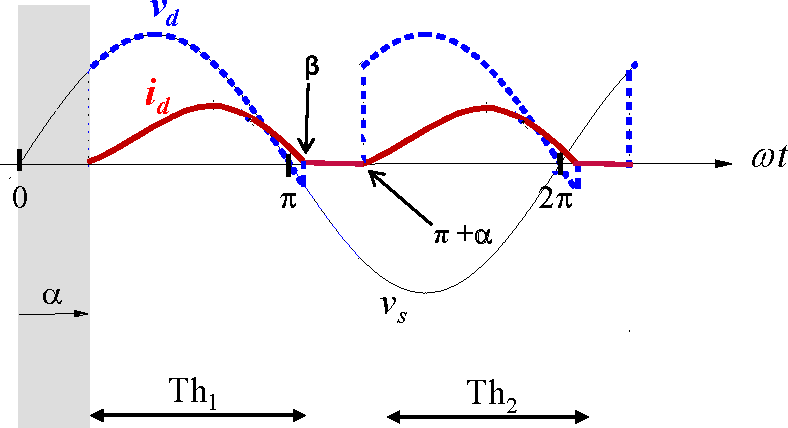
\includegraphics[width=0.8\linewidth]{dcm}
    \caption{Mode de conduction discontinue, redresseur monophasé avec lacunes de courant}
    \label{fig:dcm}
\end{figure}

Dans la Figure~\ref{fig:dcm} il y a des aucune lacune de courant, on a ainsi :
\begin{align*}
    \beta &< \pi+\alpha\\
    \phi &< \alpha
\end{align*}

\subsection{Essais expérimentaux}
Le premier essais consiste à faire varier la valeur de l'angle de déclenchement $\alpha$.

\begin{figure}[!ht]
    \centering
    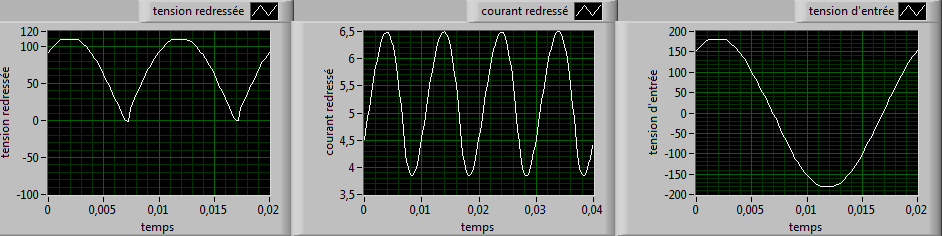
\includegraphics[width=\linewidth]{red_1_3}
    \caption{Mode de conduction continue, $\alpha=\SI{0}{\degree}$}
    \label{fig:ccm_msr}
\end{figure}

\begin{figure}[!ht]
    \centering
    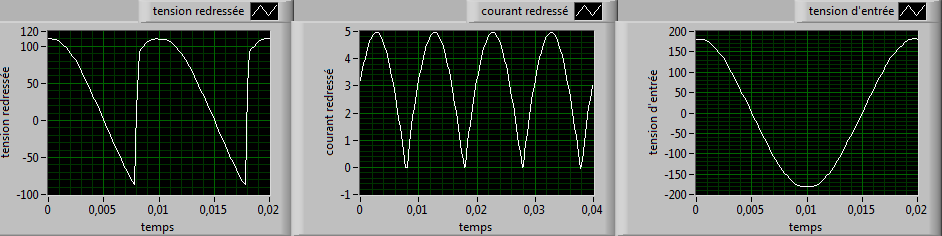
\includegraphics[width=\linewidth]{red_1_2}
    \caption{Mode de conduction continue limite, $\alpha \approx \SI{27}{\degree}$}
    \label{fig:lim_ccm_msr}
\end{figure}

\begin{figure}[!ht]
    \centering
    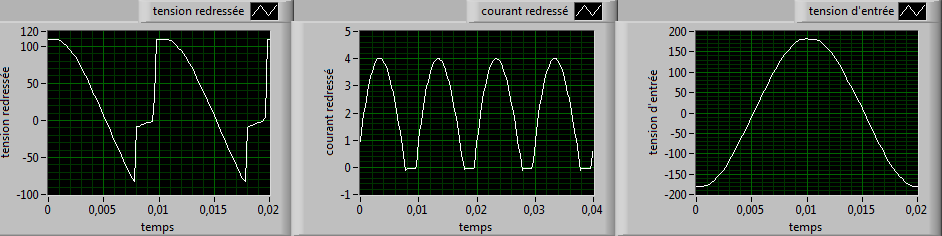
\includegraphics[width=\linewidth]{red_1_1}
    \caption{Mode de conduction discontinue, $\alpha \approx \SI{40.5}{\degree}$}
    \label{fig:dcm_msr}
\end{figure}

\clearpage
\section{Étude en redresseur triphasé à point neutre}
Nous allons ici déterminer la caractéristique externe du pont triphasé à trois thyristors. Aussi la loi d'empiètement $\mu$ en fonction du courant moyen $I_d$ pour des valeur de $\alpha$ égales à $\SI{0}{\degree}$, $\SI{30}{\degree}$. Finalement nous ferons varier la valeur de l'angle $\alpha$ en gardant $I_d=\SI{10}{\ampere}$ tout en relevant la puissance active au primaire du transformateur d'alimentation.

\subsection{Théorie \label{subsec:th2}}

\begin{figure}[!ht]
    \centering
    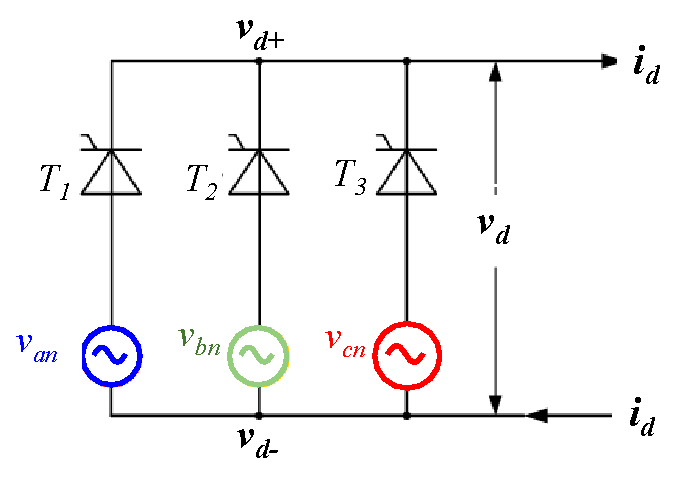
\includegraphics[width=0.8\linewidth]{cir_tripha}
    \caption{Circuit triphasé, point neutre}
    \label{fig:cir_tripha}
\end{figure}

Ce circuit consiste en la mise en parallèle de 3 thyristors sur les phases a, b et c. Le thyristor ayant la tension $v_{d+}$ la plus positive conduira. La Figure~\ref{fig:tri_wave} montre le fonctionnement avec un angle d'allumage $\alpha=\SI{0}{\degree}$.

\clearpage
\begin{figure}[!ht]
    \centering
    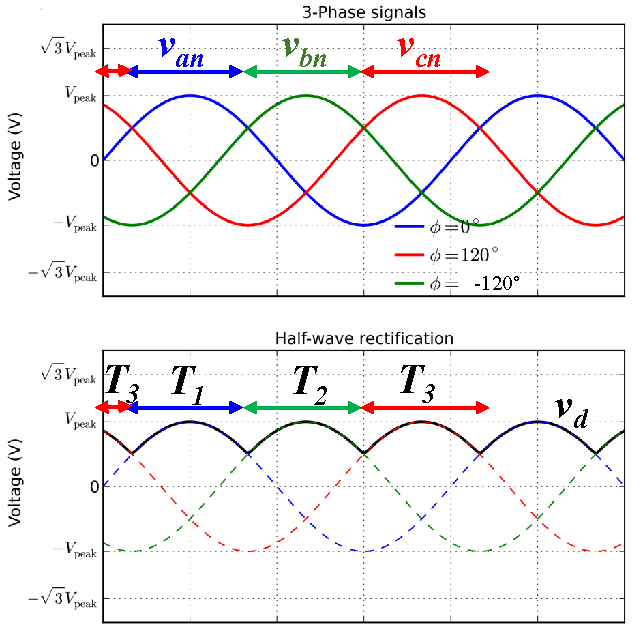
\includegraphics[width=0.8\linewidth]{tri_func}
    \caption{Fonctionnement du circuit triphasé, point neutre, $\alpha=\SI{0}{\degree}$}
    \label{fig:tri_wave}
\end{figure}

Nous connaissons l'expression des tensions étoilées $v_{an}$, $v_{bn}$ et $v_{cn}$ :

\begin{align*}
 v_{an} &= \sqrt{2} \cdot \sin{\left(\omega \cdot t\right)}\phantom{\left( ( \dfrac{2\pi}{3}\right)} \quad \rightarrow \quad \underline{V_{an}} = V_s\\
 v_{bn} &= \sqrt{2} \cdot \sin{\left(\omega \cdot t - \dfrac{2\pi}{3}\right)} \quad \rightarrow \quad \underline{V_{bn}} = \underline{V_{an}} \cdot e^{-\jmath \dfrac{2\pi}{3}}\\
 v_{cn} &= \sqrt{2} \cdot \sin{\left(\omega \cdot t + \dfrac{2\pi}{3}\right)} \quad \rightarrow \quad \underline{V_{cn}} = \underline{V_{an}} \cdot e^{\jmath \dfrac{2\pi}{3}}
 \end{align*}
 
 \clearpage
 Dans le cas d'une charge fortement inductive nous obtenons les graphiques suivants pour différentes valeurs de $\alpha$:
\begin{figure}[!ht]
    \centering
    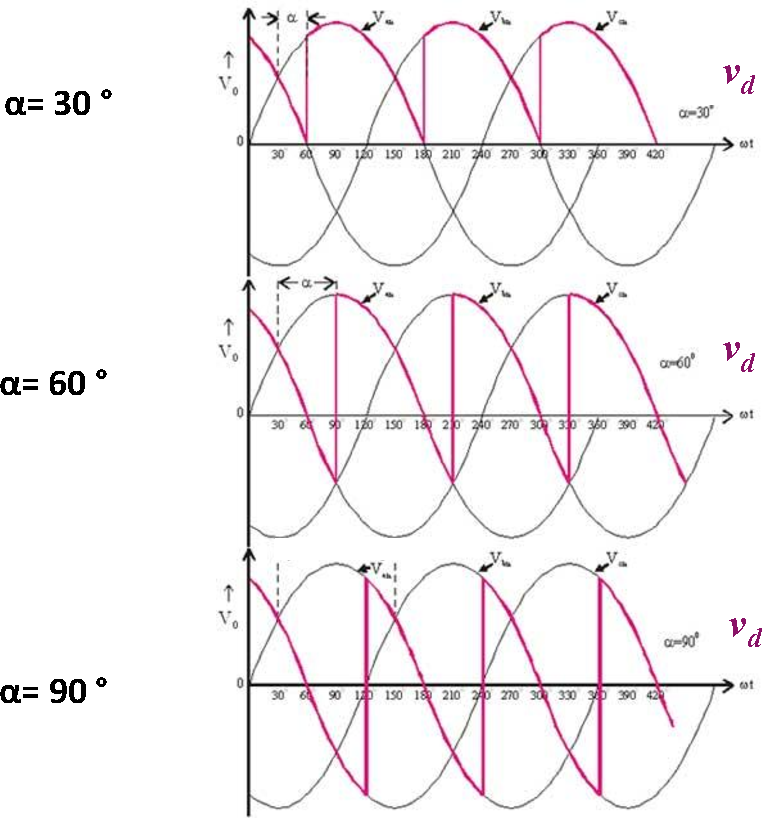
\includegraphics[width=0.8\linewidth]{alpha_30_60_90}
    \caption{Tension redressée dans un convertisseur triphasée pour différentes valeurs de $\alpha$}
    \label{fig:tri_wave_var_alpha}
\end{figure}

Jusqu'à présent, nous avons négligé la valeur d'empiètement $\mu$. Cette valeur représente l'angle qui apparaît quand le transfert de courant n'est pas instantanée entre une voie vers une autre. Lors du phénomène, deux transistors conduisent au même moment induisant une chute de tension dû à l'empiètement comme le montre la Figure~\ref{fig:mu_empiet} :

\begin{figure}[!ht]
    \centering
    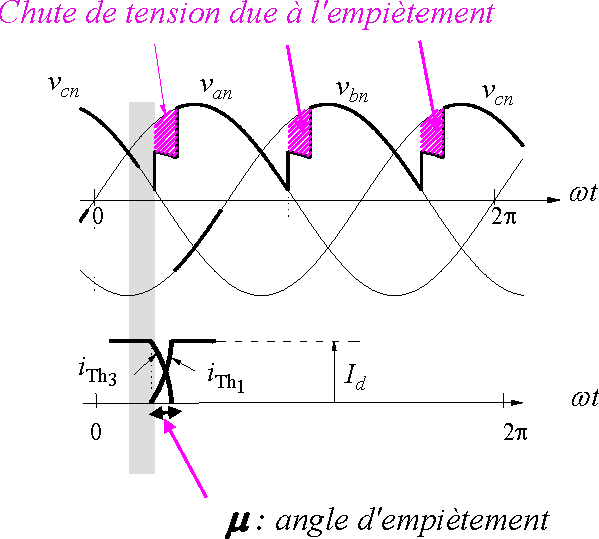
\includegraphics[width=0.8\linewidth]{empiet}
    \caption{Tension redressée avec la chute due à l'empiètement}
    \label{fig:mu_empiet}
\end{figure}

La chute de tension due à l'empiètement (voir Figure~\ref{fig:mu_empiet}) engendre un valeur de tension redressée instantanée plus basse qui s'exprime comme suit :

\begin{align*}
    v_d = \dfrac{v_{an} + v_{cn}}{2}
\end{align*}

La chute de tension est due à $L_S$ et est décrite par la relation suivante :

\begin{align*}
    V_d = V_{d\alpha} - \Delta V_{d\mu} - \Delta V_R - \Delta V_{THy} \qquad \left(V_d = f\left(I_d\right)\right)
\end{align*}

Où :

\begin{description}
\item[$V_d$] est la tension moyenne redressée
\item[$V_{d\alpha}$] est la tension moyenne redressée, cas idéal
\item[$\Delta V_{d\mu}$] est la chute de tension par empiétement, pris en compte de $L_S$
\item[$\Delta V_R$] est la chute de tension due à la résistance interne de la source
\item[$\Delta V_{THy}  = V_{\text{on}}$] est la chute de tension par thyristor, au cours de la conduction
\end{description}

Les différents termes listés précédemment sont exprimés comme suit :

\begin{align*}
    V_{d\alpha} &= \dfrac{3\sqrt{2}}{2\pi} \cdot V_L \cdot \cos{\left(\alpha \right)}\\
    \Delta V_{d\mu} &= \dfrac{3}{2\pi} \cdot \omega \cdot L_S \cdot I_d\\
    \Delta V_R &= \left(R_2 + m^2 \cdot R_1 \right)\cdot I_d\\
    \Delta V_{THy} &= 0,8 + 0,04 \cdot I_d\\
    L_S &= L_2 + L_1 \cdot m^2\\
    m &= \dfrac{V_{L_2}}{V_{L_1}}
\end{align*}

Où :

\begin{description}
\item[$V_L$] est la valeur efficace de la tension de ligne (phase à phase) côté secondaire ($V_{L_2}$)
\item[$L_1$, $L_2$] sont les inductances de dispersion du primaire et du secondaire du transformateur
\item[$R_1$, $R_2$] sont les résistances de dispersion du primaire et du secondaire du transformateur
\item[$m$] est le rapport de transformation
\end{description}

\subsection{Essais expérimentaux}
\subsubsection{Caractéristique externe quand $\alpha = \SI{0}{\degree}$}
Dans cet essai, la tension de ligne au primaire est de \SI{130}{\volt}. La résistance variable va nous permettre de faire varier la valeur du courant $I_d$ qui traverse la charge résistive du pont redresseur. Nous relèverons les valeurs du courant $I_d$, de la tension $V_d$ et de l'angle d'empiètement $\mu$ (mesuré à l'oscilloscope) avec une valeur de $\alpha$ nulle. Il faut note que la valeur de $\mu$ sera relevé en \si{\mu\s}, or à \SI{50}{\hertz}, $\SI{1}{\mu\s}$ correspond à \SI{0.018}{\degree} ($\SI{360}{\degree} \times \SI{50}{\hertz} / 10^6$).

\begin{table}[!ht]
\centering
\begin{tabular}{llll}
\toprule
$I_d$ [\si{\ampere}] & $V_d$ [\si{\volt}] & $t_{commutation}$ [\si{\mu\s}] & $\mu$ [\si{\degree}] \\
\midrule
0         & 94,25        & /                           & /                          \\
3         & 93,55        & 351                         & 6,318                      \\
6         & 92,4         & 537                         & 9,666                      \\
9         & 91,38        & 682                         & 12,276                     \\
12        & 90,26        & 793                         & 14,274                     \\
15        & 89,48        & 902                         & 16,236                     \\
18        & 88,57        & 998                         & 17,964                     \\
21        & 87,5         & 1056                        & 19,008                     \\
24        & 86,25        & 1186                        & 21,348                     \\
27        & 85,6         & 1252                        & 22,536                     \\
30        & 84,8         & 1350                        & 24,3                       \\
\bottomrule
\end{tabular}
\caption{Mesures pour $\alpha = \SI{0}{\degree}$}
\end{table}

\begin{figure}[!ht]
    \centering
    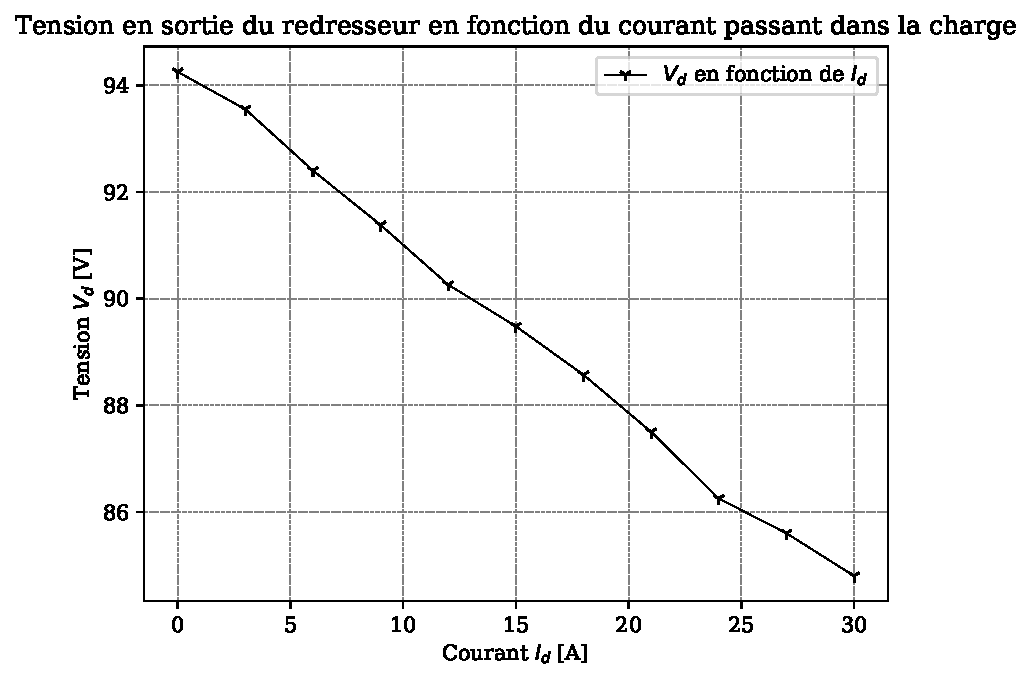
\includegraphics[width=0.8\linewidth]{exp1_graph1}
    \caption{Caractéristique externe $V_d=f\left(I_d\right)$ avec $\alpha = \SI{0}{\degree}$}
    \label{fig:exp1grap1}
\end{figure}

Afin d'augmenter la valeur du courant dans la charge, il est nécessaire d'abaisser la valeur de la résistance. La valeur de $V_{d\alpha}$ est constante et est égale à \SI{130}{\volt}. Il en découle que quand le courant passant au travers de la charge augmente, une chute de tension apparaît est la valeur de $V_d$ diminue. Ici, dans la Figure~\ref{fig:exp1grap1} on constate que la relation est quasi linéaire et proportionnelle à $I_d$.

\begin{figure}[!ht]
    \centering
    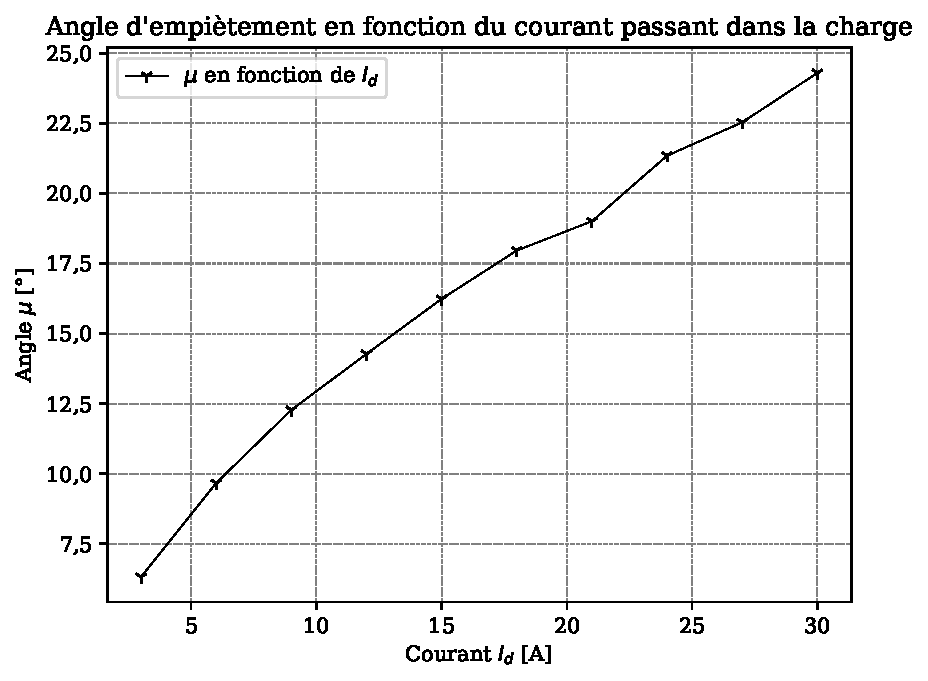
\includegraphics[width=0.8\linewidth]{exp1_graph2}
    \caption{Loi d'empiètement en fonction du courant de charge $\mu=f\left(I_d\right)$ avec $\alpha = \SI{0}{\degree}$}
    \label{fig:exp1grap2}
\end{figure}

Concernant la loi d'empiétement (Figure~\ref{fig:exp1grap2}), on constate que l'empiètement augmente avec la valeur du courant $I_d$. Les relations qui expriment $\mu$ sont les suivantes :

\begin{align*}
    \cos{\left(\alpha + \mu\right)} &= \cos{\left(\alpha \right)} - \dfrac{2 \omega L_S}{\sqrt{2} \cdot V_L} \cdot I_d\\
    \mu &= \arccos{\left(\cos{\left(\alpha \right)} - \dfrac{2 \omega L_S}{\sqrt{2} \cdot V_L}\cdot I_d\right)} - \alpha
\end{align*}

Dès lors, quand $I_d$ augmente, l'argument de l'arc-cosinus diminue et donc la valeur de l'arc-cosinus augmente.

\clearpage
\subsubsection{Caractéristique externe quand $\alpha = \SI{30}{\degree}$}

Dans cet essai, la valeur de $\alpha$ est égale à \SI{30}{\degree}. Avec cette valeur, les lacunes de courant apparaissent, engendrant des justes de tension supplémentaires.

\begin{table}[!ht]
\centering
\begin{tabular}{llll}
\toprule
$I_d$ [\si{\ampere}] & $V_d$ [\si{\volt}] & $t_{commutation}$ [\si{\mu\s}] & $\mu$ [\si{\degree}] \\
\midrule
0         & 82,26        & /                           & /                          \\
3         & 81,78        & 55,2                        & 0,9936                     \\
6         & 80,43        & 107,4                       & 1,9332                     \\
9         & 79,62        & 155                         & 2,79                       \\
12        & 78,31        & 207                         & 3,726                      \\
15        & 77,4         & 256                         & 4,608                      \\
18        & 76,55        & 302,6                       & 5,4468                     \\
21        & 75,62        & 354                         & 6,372                      \\
24        & 74,22        & 396,8                       & 7,1424                     \\
27        & 73,9         & 437,4                       & 7,8732                     \\
30        & 72,7         & 490,6                       & 8,8308                     \\
\bottomrule
\end{tabular}
\caption{Mesures pour $\alpha = \SI{30}{\degree}$}
\end{table}

\begin{figure}[!ht]
    \centering
    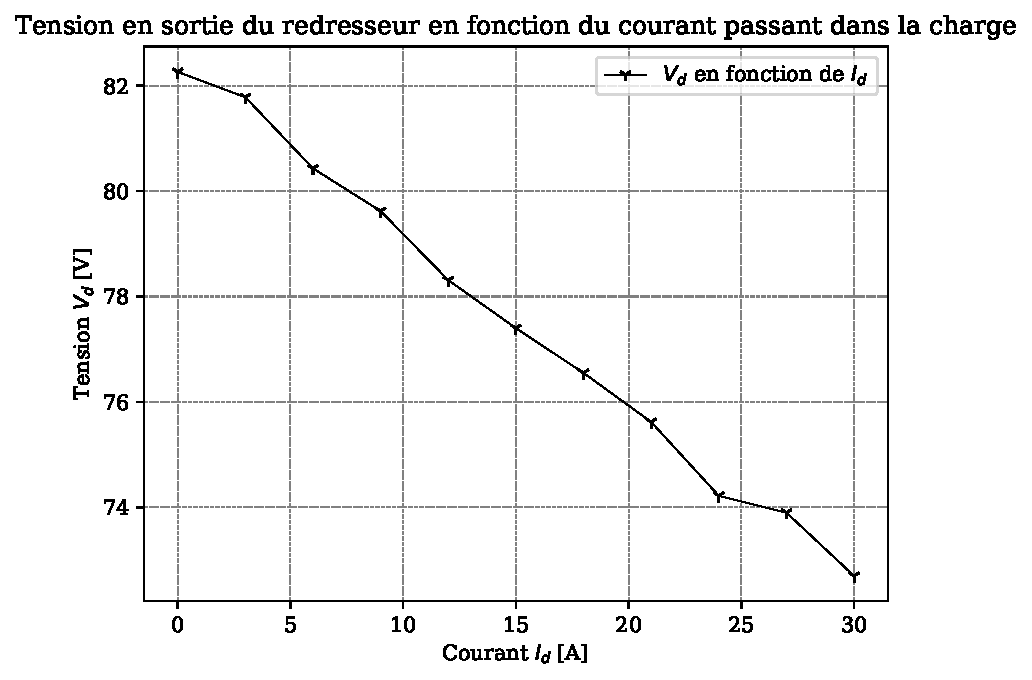
\includegraphics[width=0.8\linewidth]{exp1_graph3}
    \caption{Caractéristique externe $V_d=f\left(I_d\right)$ avec $\alpha = \SI{30}{\degree}$}
    \label{fig:exp1grap3}
\end{figure}

Comparé à la Figure~\ref{fig:exp1grap1} avec $\alpha = \SI{0}{\degree}$, la Figure~\ref{fig:exp1grap3} avec $\alpha = \SI{30}{\degree}$ montre des chutes de tension plus importantes, dues au nouveau terme introduit par les lacunes de courant. On a donc un chute de tension dans la bobine $L_S$, qui engendre une augmentation de la valeur du terme $\Delta V_{d\mu}$.

\begin{figure}[!ht]
    \centering
    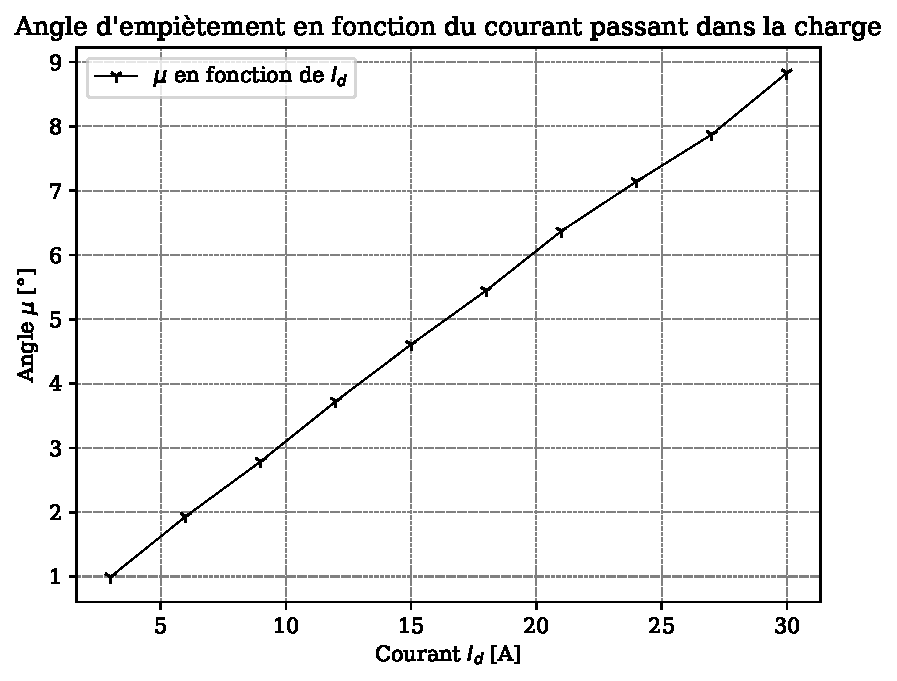
\includegraphics[width=0.8\linewidth]{exp1_graph4}
    \caption{Loi d'empiètement, fonction du courant de charge $\mu=f\left(I_d\right)$ avec $\alpha = \SI{30}{\degree}$}
    \label{fig:exp1grap4}
\end{figure}

À l'instar de la Figure~\ref{fig:exp1grap2} où $\alpha = \SI{0}{\degree}$, la Figure~\ref{fig:exp1grap4} où $\alpha = \SI{30}{\degree}$ montre une loi d'empiètement croissante au regard de $I_d$. Cependant, la valeur de l'angle d'empiètement est moindre, ce qui est dû au fait que l'angle $\alpha$ est un terme soustractif dans l'expression de l'angle d'empiètement $\mu$.

\clearpage
\subsubsection{Évolution de la puissance active en fonction de l'angle $\alpha$}

Pour ces mesures nous avons imposé un courant $I_d$ de \SI{10}{\ampere} au travers de la charge et nous avons mesuré la puissance active $P$ tout en faisant varier la valeur de l'angle $\alpha$.

\begin{table}[!ht]
\centering
\begin{tabular}{llll}
\toprule
$\alpha$ [\si{\degree}] & $P$ [\si{\watt}]\\
\midrule
0             & 1010                  \\
10            & 1000                  \\
20            & 956                   \\
30            & 900                   \\
40            & 810                   \\
50            & 700                   \\
60            & 576                   \\
70            & 420                   \\
80            & 297                   \\
\bottomrule
\end{tabular}
\caption{Mesures pour $I_d = \SI{10}{\ampere}$}
\end{table}

\begin{figure}[!ht]
    \centering
    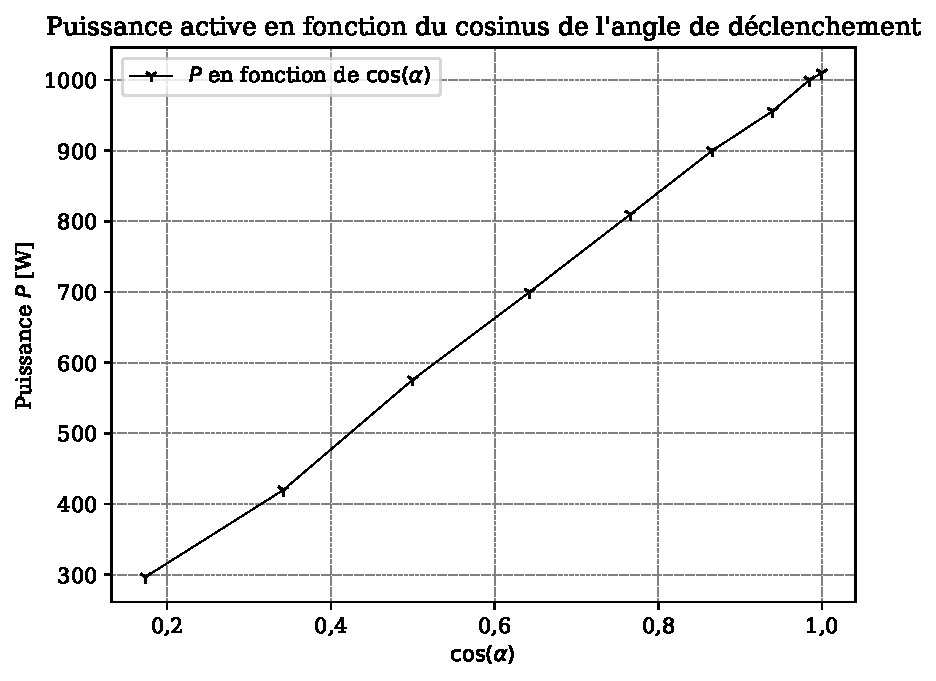
\includegraphics[width=0.8\linewidth]{exp1_graph5}
    \caption{Relevé de la puissance active en fonction de $\cos{\left(\alpha \right)}$, avec $I_d = \SI{10}{\ampere}$}
    \label{fig:exp1grap5}
\end{figure}

La valeur de la puissance active est proportionnelle à la valeur du cosinus de l'angle $\alpha$. Ce qui est appuyé par le fait que quand l'angle de retard à l'allumage des thyristors augmente, l'empiètement suit la même tendance. On a donc des chutes de tension supplémentaires et la puissance active $P$ s'en voit diminuée.

\clearpage
\subsubsection{Déterminations théoriques de la caractéristique externe et de la loi d'empiètement}

La caractéristique externe et la loi d'empiètement peuvent être déterminés théoriquement.

En reprenant dans la sous-section~\ref{subsec:th2} l'expression de la tension redressée $V_d$, nous pouvons déterminer la caractéristique externe $V_d = f\left(I_d\right)$ :

\begin{align*}
    V_d = V_{d\alpha} - \Delta V_{d\mu} - \Delta V_R - \Delta V_{THy} \qquad \left(V_d = f\left(I_d\right)\right)
\end{align*}

Le cours nous permet de déterminer la valeur de $V_{d\alpha}$. Aussi l'expression de $\underline{z}_{cc}$ permet de retrouver les expressions précédemment listées dans la sous-section~\ref{subsec:th2} ($\underline{z}_{cc}=\underline{z}_{2cc} + m^2 \cdot \underline{z}_{1cc}$).

Or on sait que $\Delta V_{THy} = 0,8 + 0,04 \cdot I_d$.

Si on considère :
\begin{align*}
    \underline{z}_{1cc} &= 0,1405 \cdot e^{\jmath \SI{56.34}{\degree}} = R_1 + \jmath \omega L_1\\
    \underline{z}_{2cc} &= 0,1530 \cdot e^{\jmath \SI{58.47}{\degree}} = R_2 + \jmath \omega L_2
\end{align*}

On obtient :

\begin{align*}
    m &= \dfrac{V_{L_2}}{V_{L_1}} = \dfrac{81 \cdot \sqrt{3}}{130} = 1,079 \\
    \omega L_S &= \omega L_2 + m^2 \omega L_1 = z_{2cc} \cdot \sin{\left(\SI{58,47}{\degree}\right)} + m^2 \cdot z_{1cc} \cdot \sin{\left(\SI{56,34}{\degree}\right)}\\
    &= 0,1530 \cdot \sin{\left(\SI{58,47}{\degree}\right)} + 1,079^2 \cdot 0,1405 \cdot \sin{\left(\SI{56,34}{\degree}\right)} \\
    &= \SI{0,26661348736989543}{} \\
    &\approx \SI{0,2666}{}
\end{align*}

Ce qui donne :
\begin{align*}
    V_{d\alpha} &= \dfrac{3\sqrt{2}}{2\pi} \cdot V_L \cdot \cos{\left(\alpha \right)} = \dfrac{3\sqrt{2}}{2\pi} \cdot 81 \sqrt{3} \cdot \cos{\left(\alpha \right)}\\
    \Delta V_{d\mu} &= \dfrac{3}{2\pi} \cdot \omega \cdot L_S \cdot I_d = \dfrac{3}{2\pi} \cdot \SI{0,2666}{} \cdot I_d\\
    \Delta V_R &= \left(R_2 + m^2 \cdot R_1 \right)\cdot I_d = \left(0,1530 \cdot \cos{\left(\SI{58.47}{\degree} \right)} + 1,079^2 \cdot 0,1405 \cdot \cos{\left(\SI{56.34}{\degree} \right)} \right)\cdot I_d\\
    &= \SI{0.17070831398559172}{}\cdot I_d\\
    &\approx \SI{0.1707}{}\cdot I_d
\end{align*}

Finalement :

\begin{align*}
    V_d &= \dfrac{3\sqrt{2}}{2\pi} \cdot 81 \sqrt{3} \cdot \cos{\left(\alpha \right)} - \SI{0.1273}{} \cdot I_d - \SI{0.1707}{}\cdot I_d - 0,8 - 0,04 \cdot I_d\\
    &= \dfrac{3\sqrt{2}}{2\pi} \cdot 81 \sqrt{3} \cdot \cos{\left(\alpha \right)} - \SI{0,338}{} \cdot I_d - 0,8
\end{align*}

Afin de déterminer l'empiétement nous reprendrons la relation précédemment montrée :

\begin{align*}
    \mu &= \arccos{\left(\cos{\left(\alpha \right)} - \dfrac{2 \omega L_S}{\sqrt{2} \cdot V_L}\cdot I_d\right)} - \alpha
\end{align*}

À l'aide des lois théoriques, nous sommes capable de comparer les mesures effectuées avec leurs valeurs théoriques calculées.

\begin{figure}[!ht]
    \centering
    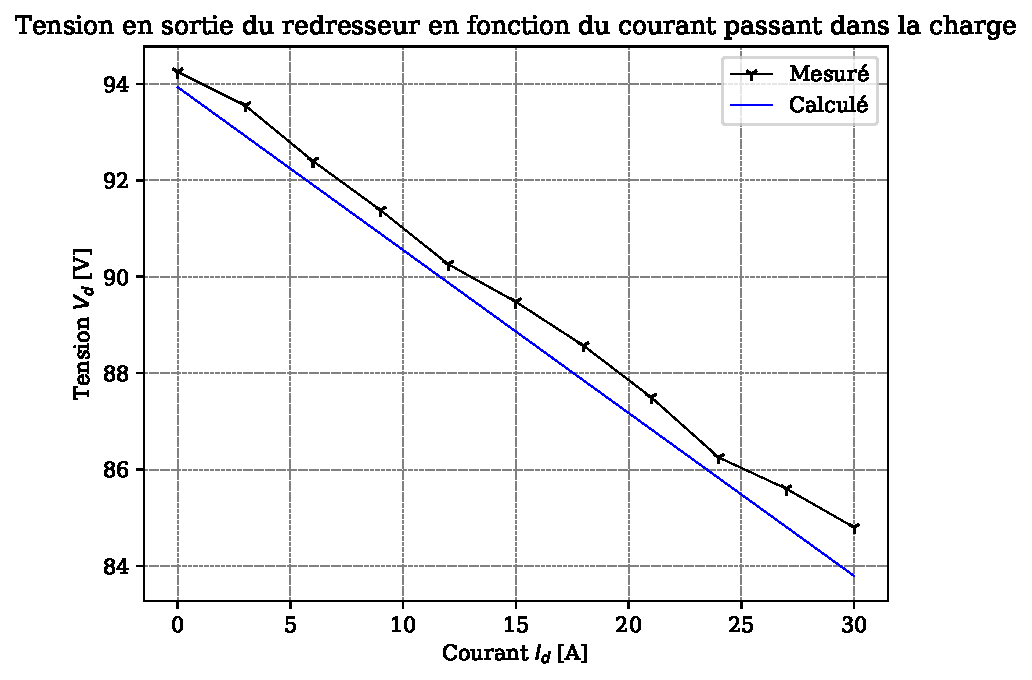
\includegraphics[width=0.8\linewidth]{exp1_graph6}
    \caption{Comparaison de la caractéristique externe $V_d=f\left(I_d\right)$ avec $\alpha = \SI{0}{\degree}$}
    \label{fig:exp1grap6}
\end{figure}

\begin{figure}[!ht]
    \centering
    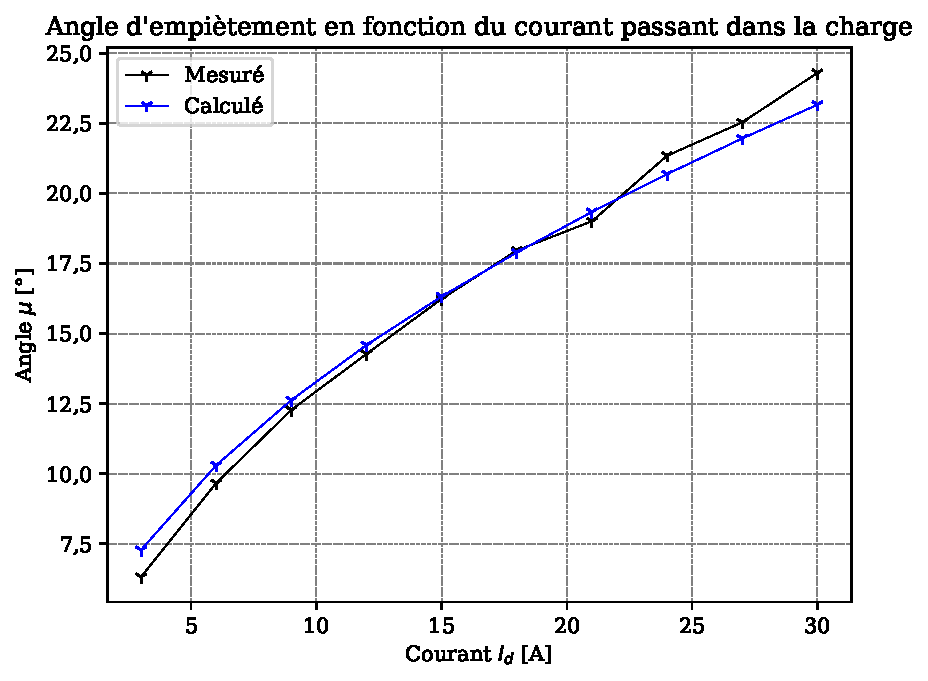
\includegraphics[width=0.8\linewidth]{exp1_graph8}
    \caption{Comparaison de la loi d'empiètement, fonction du courant de charge $\mu=f\left(I_d\right)$ avec $\alpha = \SI{0}{\degree}$}
    \label{fig:exp1grap8}
\end{figure}

Les tendances des tracés mesuré et calculé des figures (Figure~\ref{fig:exp1grap6} et Figure~\ref{fig:exp1grap8}) sont très proches, les différences sont probablement dues à des erreurs sur les mesures.

\begin{figure}[!ht]
    \centering
    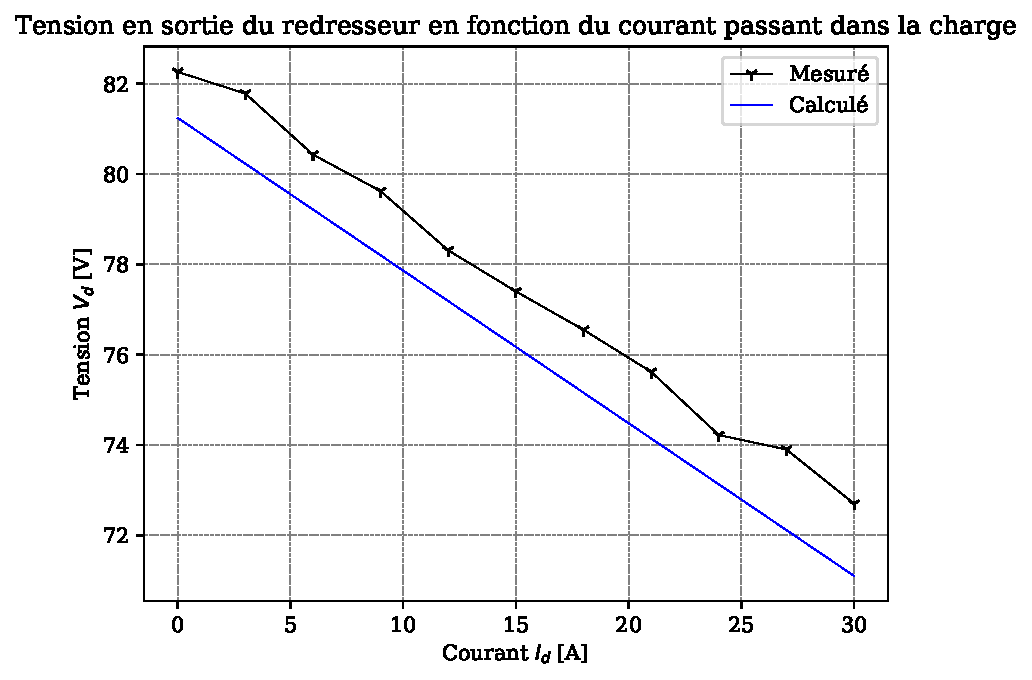
\includegraphics[width=0.8\linewidth]{exp1_graph7}
    \caption{Comparaison de la caractéristique externe $V_d=f\left(I_d\right)$ avec $\alpha = \SI{30}{\degree}$}
    \label{fig:exp1grap7}
\end{figure}
\clearpage

\begin{figure}[!ht]
    \centering
    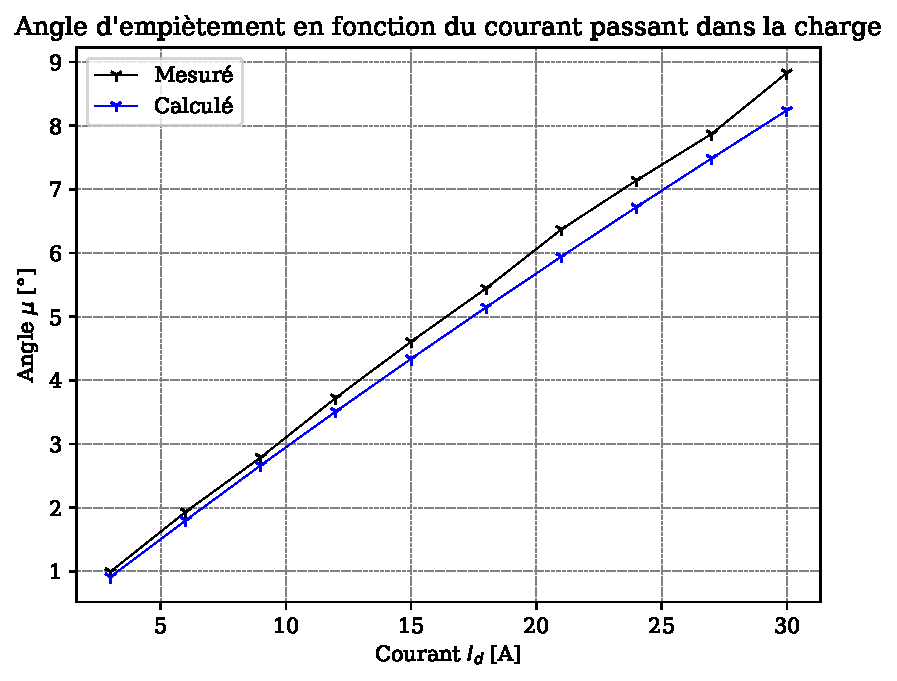
\includegraphics[width=0.8\linewidth]{exp1_graph9}
    \caption{Comparaison de la loi d'empiètement, fonction du courant de charge $\mu=f\left(I_d\right)$ avec $\alpha = \SI{30}{\degree}$}
    \label{fig:exp1grap9}
\end{figure}

À l'instar des figures précédentes, les tendances des tracés mesuré et calculé des figures (Figure~\ref{fig:exp1grap7} et Figure~\ref{fig:exp1grap9}) sont très proches, les différences sont probablement dues à des erreurs sur les mesures.

\clearpage
\section{Problème du facteur de puissance}
\subsection{Théorie}
Nous allons maintenant étudier le fonctionnement du pont de Graetz, représenté sur la Figure~\ref{fig:cir_graetz} :

\begin{figure}[!ht]
    \centering
    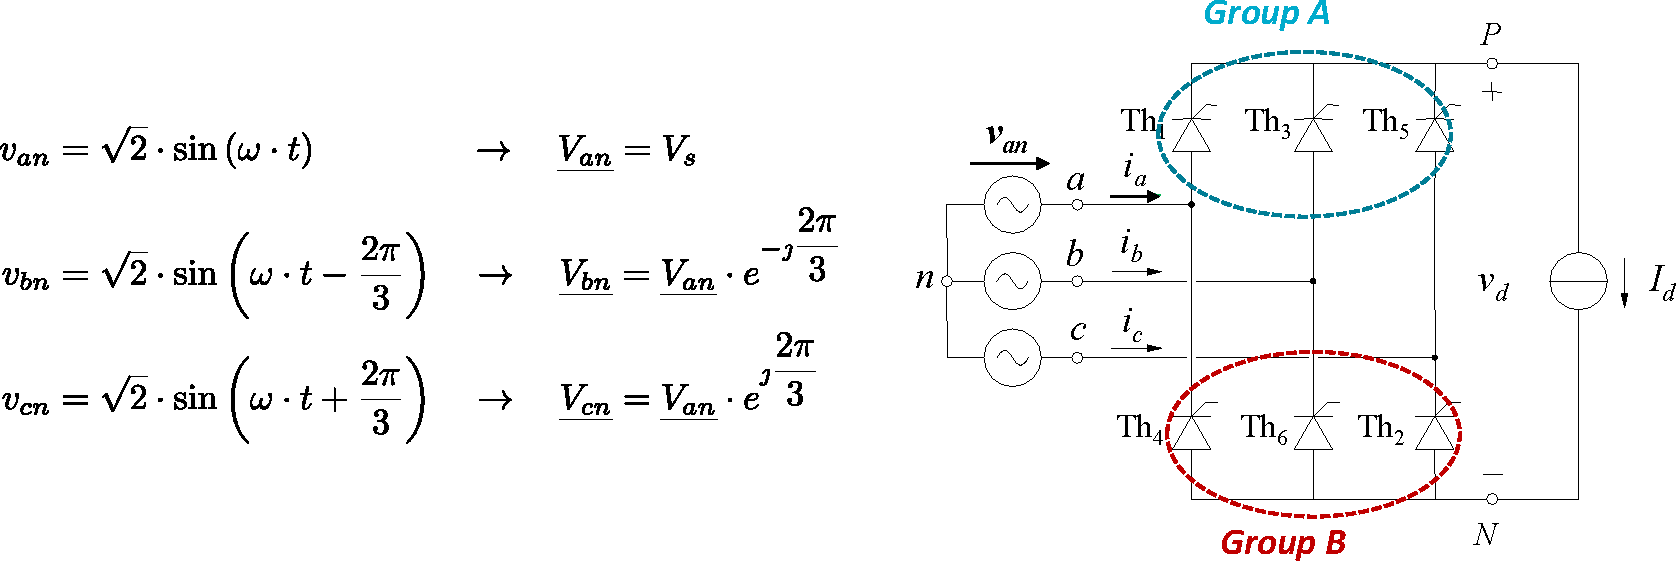
\includegraphics[width=0.8\linewidth]{graetz_tri}
    \caption{Pont de Graetz, redresseur triphasé}
    \label{fig:cir_graetz}
\end{figure}

Dans le circuit de la Figure~~\ref{fig:cir_graetz}, le groupe A est constitué des thyristors 1, 3 et 5 tandis que le groupe B est constitué des thyristors 2, 4 et 6. Le potentiel des anodes du groupe A est porté à la valeur la plus positive (ou la plus haute) de la tension, alors que le potentiel des cathodes du groupe B est porté à la valeur la plus négative (ou la plus basse).

\begin{figure}[!ht]
    \centering
    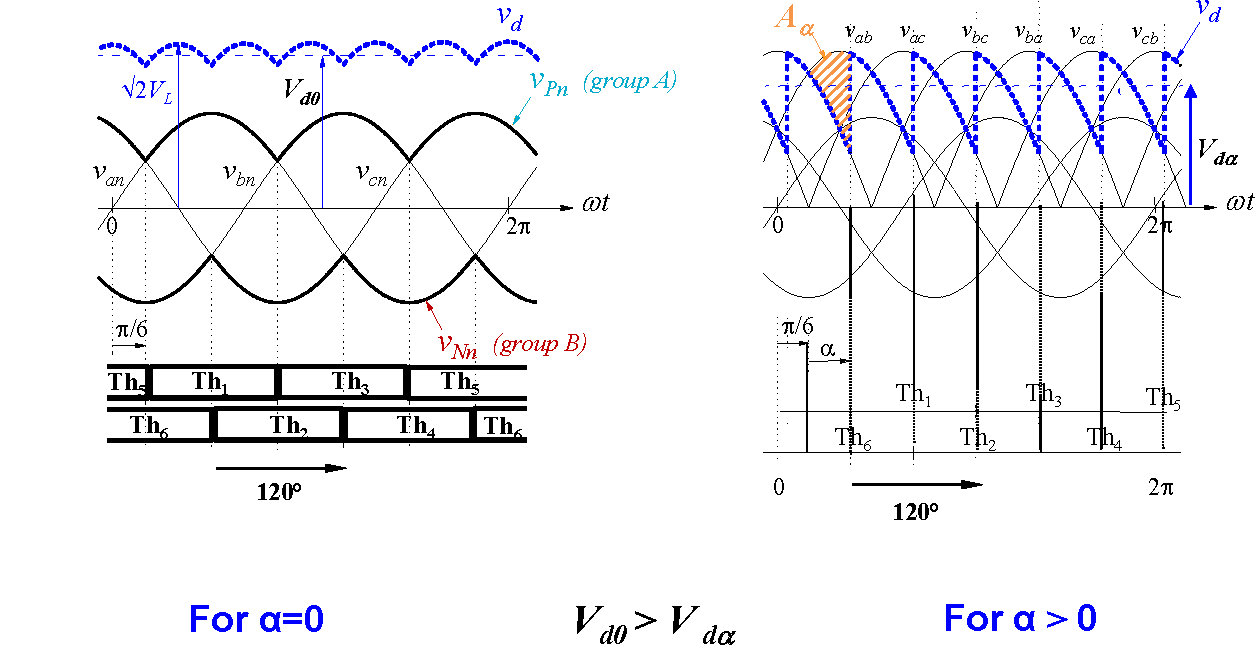
\includegraphics[width=0.8\linewidth]{graetz_wave}
    \caption{Tension redressée pour $\alpha = \SI{0}{\degree}$ et  $\alpha > \SI{0}{\degree}$}
    \label{fig:wave_graetz}
\end{figure}

La Figure~\ref{fig:wave_graetz} montre que le groupe A conduit au maxima de la tension plus positive tandis que le groupe B conduit au minima de la tension négative.

À l'instar du redresseur à point neutre, il y a un phénomène d'empiètement engendré par l'inductance de source $L_S$.

\begin{figure}[!ht]
    \centering
    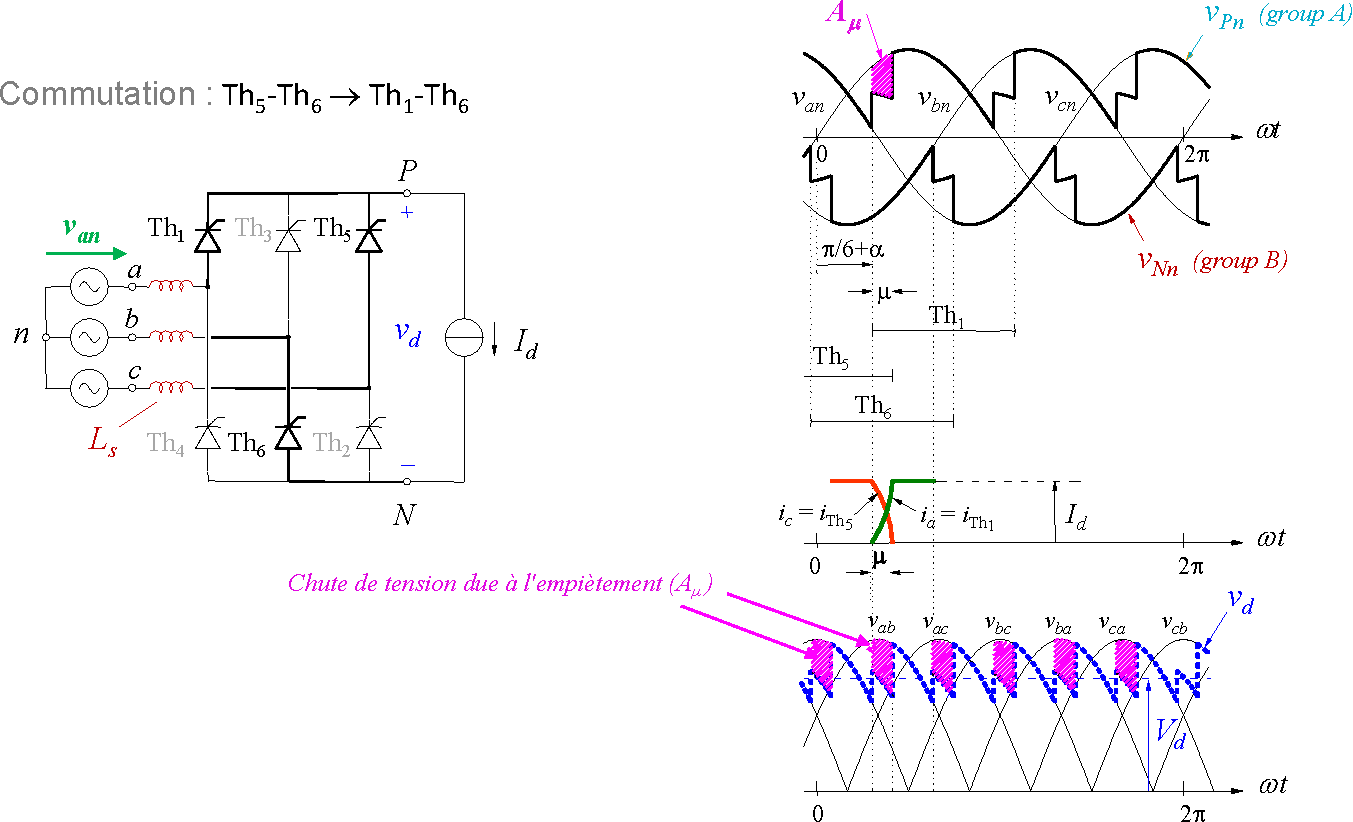
\includegraphics[width=0.8\linewidth]{graetz_empiet}
    \caption{Tension redressée en prenant en compte de l'inductance source $L_S$}
    \label{fig:empiet_graetz}
\end{figure}

La loi d'empiètement reste inchangé pour le pont de Graetz :

\begin{align*}
    \cos{\left(\alpha + \mu\right)} &= \cos{\left(\alpha \right)} - \dfrac{2 \omega L_S}{\sqrt{2} \cdot V_L} \cdot I_d
\end{align*}

\subsection{Prédéterminations}
En reprenant les formules utilisées dans le cas précédant (provenant de la sous-section~\ref{subsec:th2}) tout en n'oubliant pas d'applique un facteur 2, comme on redresse la tension sur chaque alternance.

Nous pouvons déterminer la caractéristique externe $V_d = f\left(I_d\right)$ :

\begin{align*}
    V_d = V_{d\alpha} - \Delta V_{d\mu} - \Delta V_R - \Delta V_{THy} \qquad \left(V_d = f\left(I_d\right)\right)
\end{align*}

De la même manière on peut déterminer la valeur de $V_{d\alpha}$. Aussi l'expression de $\underline{z}_{cc}$ permet de retrouver les expressions précédemment listées dans la sous-section~\ref{subsec:th2} ($\underline{z}_{cc}=\underline{z}_{2cc} + m^2 \cdot \underline{z}_{1cc}$).

Or on sait que $\Delta V_{THy} = 0,8 + 0,04 \cdot I_d$.

Si on considère :
\begin{align*}
    \underline{z}_{1cc} &= 0,1405 \cdot e^{\jmath \SI{56.34}{\degree}} = R_1 + \jmath \omega L_1\\
    \underline{z}_{2cc} &= 0,1530 \cdot e^{\jmath \SI{58.47}{\degree}} = R_2 + \jmath \omega L_2
\end{align*}

On obtient :

\begin{align*}
    m &= \dfrac{V_{L_2}}{V_{L_1}} = \dfrac{\SI{46.2}{} \cdot \sqrt{3}}{130} = 0,6155 \\
    \omega L_S &= \omega L_2 + m^2 \omega L_1 = z_{2cc} \cdot \sin{\left(\SI{58,47}{\degree}\right)} + m^2 \cdot z_{1cc} \cdot \sin{\left(\SI{56,34}{\degree}\right)}\\
    &= 0,1530 \cdot \sin{\left(\SI{58,47}{\degree}\right)} + 0,6155^2 \cdot 0,1405 \cdot \sin{\left(\SI{56,34}{\degree}\right)} \\
    &= \SI{0.17471514445113714}{} \\
    &\approx \SI{0.1747}{}
\end{align*}

Ce qui donne :
\begin{align*}
    V_{d\alpha} &= \dfrac{3\sqrt{2}}{\pi} \cdot V_L \cdot \cos{\left(\alpha \right)} = \dfrac{3\sqrt{2}}{\pi} \cdot 46,2 \cdot \sqrt{3} \cdot \cos{\left(\alpha \right)}\\
    \Delta V_{d\mu} &= \dfrac{3}{\pi} \cdot \omega \cdot L_S \cdot I_d = \dfrac{3}{\pi} \cdot \SI{0.1747}{} \cdot I_d\\
    \Delta V_R &= 2 \cdot \left(R_2 + m^2 \cdot R_1 \right)\cdot I_d = 2 \cdot \left(0,1530 \cdot \cos{\left(\SI{58.47}{\degree} \right)} + 0,6155^2 \cdot 0,1405 \cdot \cos{\left(\SI{56.34}{\degree} \right)} \right)\cdot I_d\\
    &= \SI{0.21902477540509432}{}\cdot I_d\\
    &\approx \SI{0.2190}{}\cdot I_d
\end{align*}

Finalement :

\begin{align*}
    V_d &= \dfrac{3\sqrt{2}}{\pi} \cdot 46,2 \cdot \sqrt{3} \cdot \cos{\left(\alpha \right)} - \SI{0.1668}{} \cdot I_d - \SI{0.2190}{}\cdot I_d - 1,6 - 0,08 \cdot I_d\\
    &= \dfrac{3\sqrt{2}}{\pi} \cdot 46,2 \cdot \sqrt{3} \cdot \cos{\left(\alpha \right)} - \SI{0.4658}{} \cdot I_d - 1,6
\end{align*}

Afin de déterminer l'empiétement nous reprendrons la relation précédemment montrée :

\begin{align*}
    \mu &= \arccos{\left(\cos{\left(\alpha \right)} - \dfrac{2 \omega L_S}{\sqrt{2} \cdot V_L}\cdot I_d\right)} - \alpha
\end{align*}

À l'aide des lois théoriques, nous sommes capable de comparer les mesures effectuées avec leurs valeurs théoriques calculées.

\clearpage
\subsection{Essais expérimentaux}
\subsubsection{Relevés de la tension redressée et de l'angle d'empiètement pour $\alpha = \SI{0}{\degree}$}

\begin{table}[!ht]
\centering
\begin{tabular}{llll}
\toprule
$I_d$ [\si{\ampere}] & $V_d$ [\si{\volt}] & $t_{commutation}$ [\si{\mu\s}] & $\mu$ [\si{\degree}] \\
\midrule
0         & 107,5        & /                           & /                          \\
3         & 107,1        & 283,2                       & 5,0976                     \\
6         & 106          & 402                         & 7,236                      \\
9         & 104,6        & 508,4                       & 9,1512                     \\
12        & 103,7        & 584,4                       & 10,5192                    \\
15        & 102,8        & 663,6                       & 11,9448                    \\
18        & 101,7        & 754                         & 13,572                     \\
21        & 100,9        & 798,8                       & 14,3784                    \\
24        & 99,8         & 879,6                       & 15,8328                    \\
27        & 99           & 940,4                       & 16,9272                    \\
30        & 98,4         & 1001,2                      & 18,0216                    \\
\bottomrule
\end{tabular}
\caption{Mesures pour $\alpha = \SI{0}{\degree}$}
\end{table}

\begin{figure}[!ht]
    \centering
    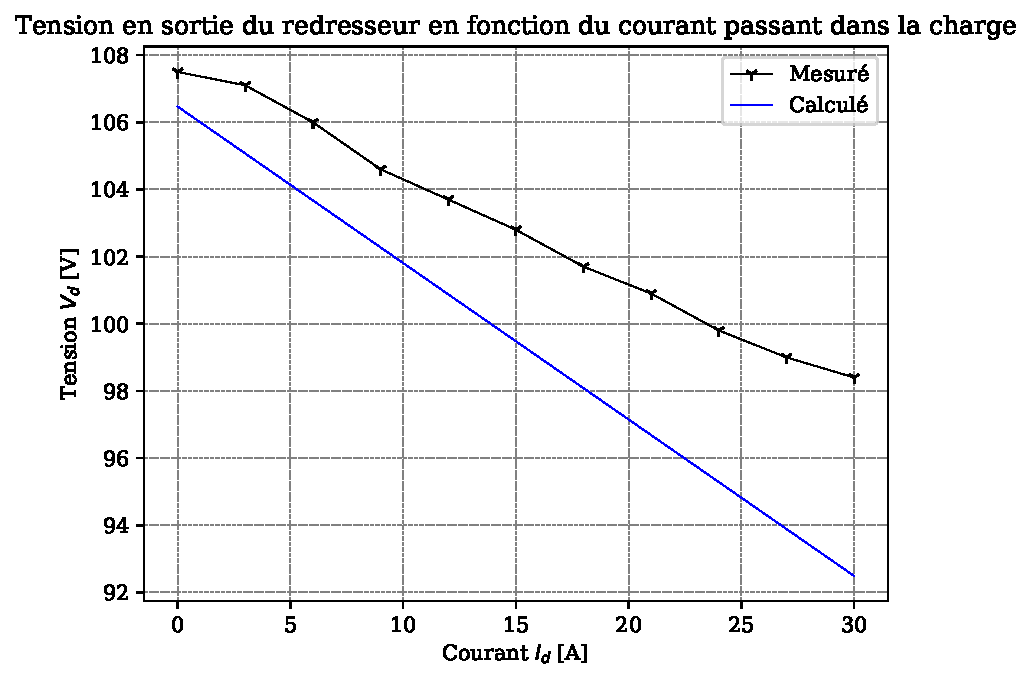
\includegraphics[width=0.8\linewidth]{exp1_graph10}
    \caption{Comparaison de la caractéristique externe $V_d=f\left(I_d\right)$ avec $\alpha = \SI{0}{\degree}$}
    \label{fig:exp1grap10}
\end{figure}
\clearpage

\begin{figure}[!ht]
    \centering
    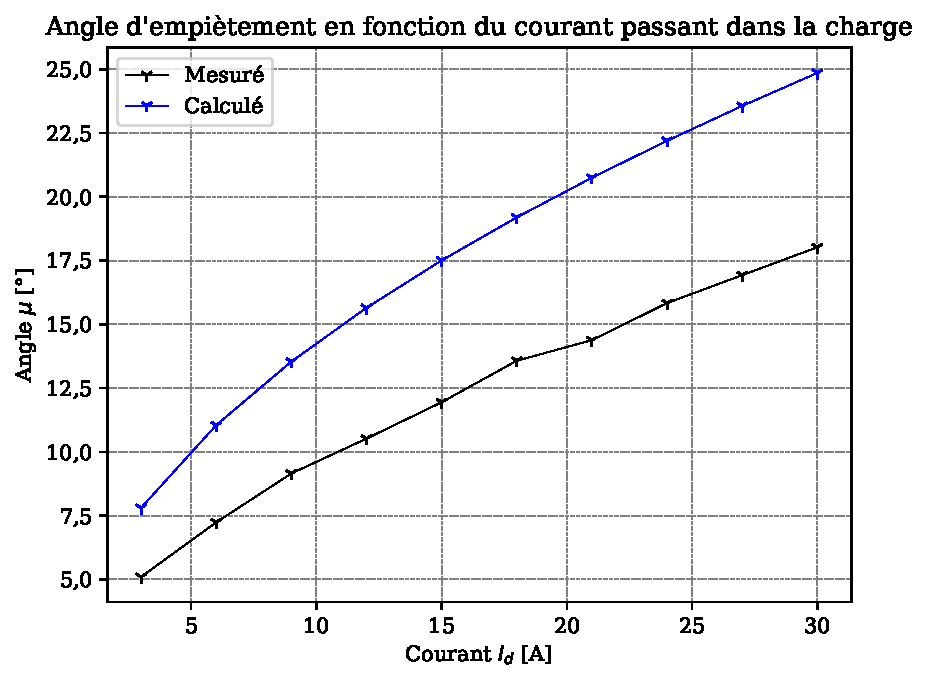
\includegraphics[width=0.8\linewidth]{exp1_graph11}
    \caption{Comparaison de la loi d'empiètement, fonction du courant de charge $\mu=f\left(I_d\right)$ avec $\alpha = \SI{0}{\degree}$}
    \label{fig:exp1grap11}
\end{figure}
 
À l'instar des cas précédents, les tendances sont assez semblables, bien qu'ici l'on constate que la pente de la prévision est plus prononcée que celle de la mesure réalisée pour la mesure de la caractéristique externe. En ce qui concerne l'empiètement, on constate un léger décalage, mais la tendance semble identique. Les erreurs sur les mesures et la qualité du modèle utilisé peuvent expliquer ces différences.
 
\clearpage
\subsubsection{Relevés de la tension redressée et de l'angle d'empiètement pour $\alpha = \SI{30}{\degree}$}

\begin{table}[!ht]
\centering
\begin{tabular}{llll}
\toprule
$I_d$ [\si{\ampere}] & $V_d$ [\si{\volt}] & $t_{commutation}$ [\si{\mu\s}] & $\mu$ [\si{\degree}] \\
\midrule
0         & 95           & /                           & /                          \\
3         & 94,8         & 41,34                       & 0,74412                    \\
6         & 93,5         & 71,34                       & 1,28412                    \\
9         & 94,4         & 98,2                        & 1,7676                     \\
12        & 93,9         & 126,96                      & 2,28528                    \\
15        & 92,7         & 158,2                       & 2,8476                     \\
18        & 91,8         & 190,7                       & 3,4326                     \\
21        & 91,4         & 215,3                       & 3,8754                     \\
24        & 90,3         & 251,3                       & 4,5234                     \\
27        & 89,3         & 276                         & 4,968                      \\
30        & 88,2         & 301,4                       & 5,4252                     \\
\bottomrule
\end{tabular}
\caption{Mesures pour $\alpha = \SI{30}{\degree}$}
\end{table}

\begin{figure}[!ht]
    \centering
    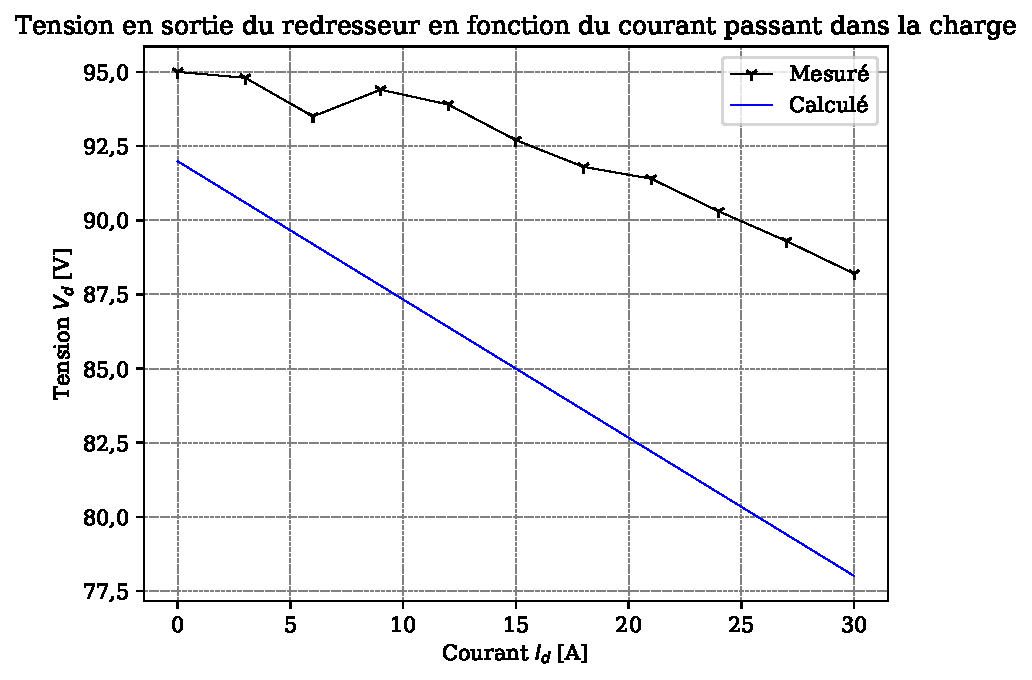
\includegraphics[width=0.8\linewidth]{exp1_graph12}
    \caption{Comparaison de la caractéristique externe $V_d=f\left(I_d\right)$ avec $\alpha = \SI{30}{\degree}$}
    \label{fig:exp1grap12}
\end{figure}
\clearpage

\begin{figure}[!ht]
    \centering
    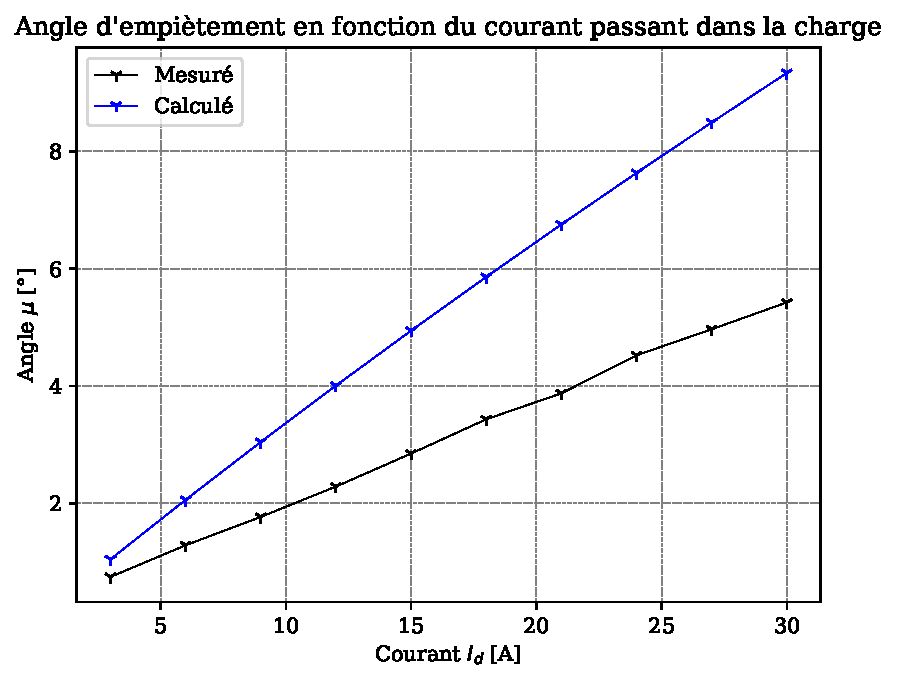
\includegraphics[width=0.8\linewidth]{exp1_graph13}
    \caption{Comparaison de la loi d'empiètement, fonction du courant de charge $\mu=f\left(I_d\right)$ avec $\alpha = \SI{30}{\degree}$}
    \label{fig:exp1grap13}
\end{figure}

Ici encore, les tendances sont assez semblables, bien qu'ici l'on constate que la pente de la prévision est plus prononcée que celle de la mesure réalisée pour la mesure de la caractéristique externe. En ce qui concerne l'empiètement, on constate une tendance légèrement différente. De même, les erreurs sur les mesures et la qualité du modèle utilisé peuvent expliquer ces différences.

\clearpage
\subsubsection{Relevé des puissances actives et réactives pour un courant de \SI{10}{\ampere} et une valeur de $\alpha$ variable}

\begin{table}[!ht]
\centering
\begin{tabular}{lll}
\toprule
$\alpha$ [$\si{\degree}$] & $P$ [$\si{\watt}$] & $Q$ [$\si{\voltampere}$] \\ \midrule
0                         & 1170               & 624                      \\
10                        & 1166               & 688                      \\
20                        & 1123               & 882                      \\
30                        & 1064               & 994                      \\
40                        & 978                & 1152                     \\
50                        & 851                & 1330                     \\
60                        & 698                & 1456                     \\
70                        & 531                & 1540                     \\
80                        & 341                & 1615                     \\
81,9                      & 299                & 1601                     \\ \bottomrule
\end{tabular}
\caption{Relevé des puissances actives et réactives pour le pont de Graetz à $\alpha$ variable et courant constant ($I_d=\SI{10}{\ampere}$)}
\end{table}

\begin{figure}[!ht]
    \centering
    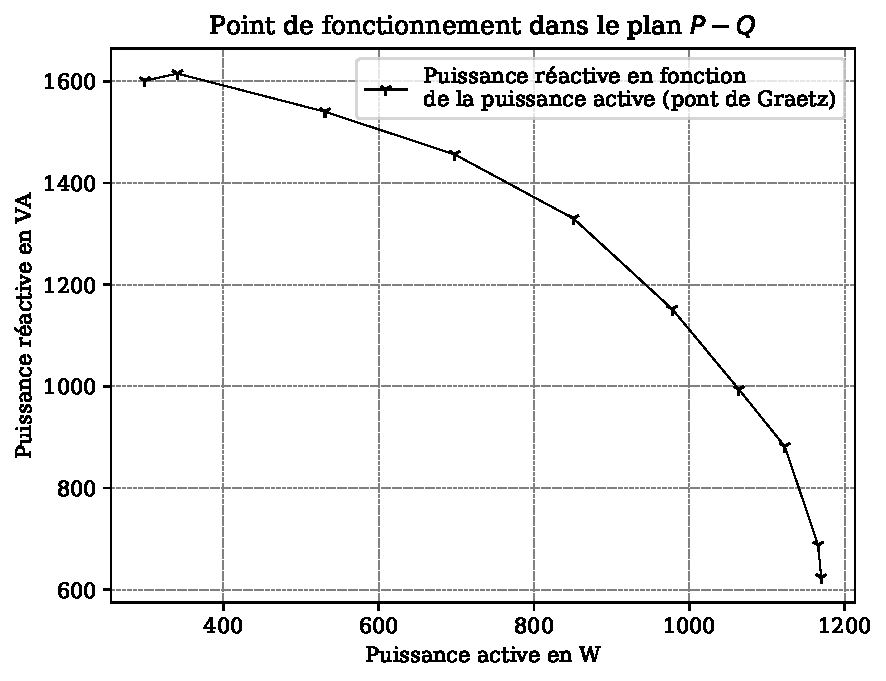
\includegraphics[width=0.8\linewidth]{exp1_graph14}
    \caption{Diagramme $P-Q$ du pont de Graetz}
    \label{fig:exp1grap14}
\end{figure}

On constate suite à l'analyse de la Figure\ref{fig:exp1grap14} que plus l'angle de retard est important et plus il y aura de puissance réactive consommée par le convertisseur au désavantage de la puissance active. Le tracé ressemble à un arc de cercle.

Pour le pont de Graetz, l'expression des puissances sont :

\begin{align*}
    P &= \sqrt{3} \cdot V_L \cdot \dfrac{\sqrt{6}}{\pi} \cdot m \cdot I_d \cdot \cos{\left(\alpha\right)}\\
    Q &= \sqrt{3} \cdot V_L \cdot \dfrac{\sqrt{6}}{\pi} \cdot m \cdot I_d \cdot \sin{\left(\alpha\right)}
\end{align*}

Dans le quart où $0 < \alpha < \frac{\pi}{2}$ on constate que quand la puissance active diminue, la puissance réactive augmente, comme la Figure\ref{fig:exp1grap14} le montre.

% \clearpage
\subsubsection{Relevé des puissances actives et réactives pour un courant de \SI{10}{\ampere} et une valeur de $\alpha$ variable sur un pont mixte}
À l'instar du relevé précédant nous allons relever les puissances actives et réactives pour un courant de \SI{10}{\ampere} et une valeur de $\alpha$ variable. Cependant, nous allons utiliser un pont mixte. C'est-à-dire un groupe de trois diodes et le second groupe sera constitué de trois thyristors. Ici pour ne pas changer de pont, on va simplement imposer un angle de retard nulle sur l'un des groupes de thyristors et faire varier $\alpha$ sur l'autre groupe.

On se retrouve donc avec un contrôle séquentiel du pont de Graetz. Les expressions des puissances actives et réactives s'écrivent alors comme suit :

\begin{align*}
    P &= \sqrt{3} \cdot V_L \cdot \dfrac{\sqrt{6}}{\pi} \cdot m \cdot I_d \cdot \cos{\left(\dfrac{\alpha_1 - \alpha_2}{2}\right)} \cdot \cos{\left(\dfrac{\alpha_1 + \alpha_2}{2}\right)}\\
    Q &= \sqrt{3} \cdot V_L \cdot \dfrac{\sqrt{6}}{\pi} \cdot m \cdot I_d \cdot \sin{\left(\dfrac{\alpha_1 - \alpha_2}{2}\right)} \cdot \sin{\left(\dfrac{\alpha_1 + \alpha_2}{2}\right)}
\end{align*}

On peut donc simplifier ces expressions comme suit avec $\alpha_1 = \SI{0}{\degree}$

\begin{align*}
    P &= \sqrt{3} \cdot V_L \cdot \dfrac{\sqrt{6}}{\pi} \cdot m \cdot I_d \cdot \left(1 + \cos{\left(\alpha_2\right)}\right)\\
    Q &= \sqrt{3} \cdot V_L \cdot \dfrac{\sqrt{6}}{\pi} \cdot m \cdot I_d \cdot \sin{\left(\alpha_2\right)}
\end{align*}

En utilisant les expressions théoriques des puissances pour le pont de Graetz et le pont mixe, nous obtenons le diagramme de la Figure~\ref{fig:comp_circle}.

\begin{figure}[!ht]
    \centering
    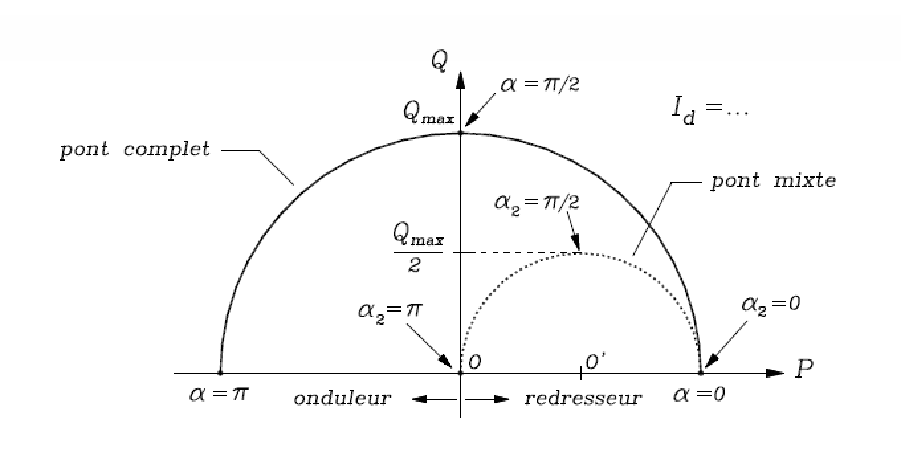
\includegraphics[width=0.8\linewidth]{circle}
    \caption{Diagramme $P-Q$ théorique pour le pont de Graetz et pour le pont mixte}
    \label{fig:comp_circle}
\end{figure}

Nous obtenons donc les valeurs suivantes (voir tableau~\ref{tab:power_mixte}).

\begin{table}[!ht]
\centering
\begin{tabular}{lll}
\toprule
$\alpha$ [$\si{\degree}$] & $P$ [$\si{\watt}$] & $Q$ [$\si{\voltampere}$] \\ \midrule
0                         & 1171               & 591                      \\
10                        & 1164               & 622                      \\
20                        & 1146               & 685                      \\
30                        & 1110               & 781                      \\
40                        & 1054               & 856                      \\
50                        & 995                & 934                      \\
60                        & 922                & 1002                     \\
70                        & 817                & 1063                     \\
80                        & 733                & 1104                     \\
90                        & 633                & 1122                     \\
100                       & 541                & 1112                     \\
110                       & 453                & 1054                     \\
120                       & 361                & 1044                     \\
129,6                     & 292                & 1009                     \\ \bottomrule
\end{tabular}
\caption{Relevé des puissances actives et réactives pour le pont mixte à $\alpha$ variable et courant constant ($I_d=\SI{10}{\ampere}$)\label{tab:power_mixte}}
\end{table}

\clearpage

\begin{figure}[!ht]
    \centering
    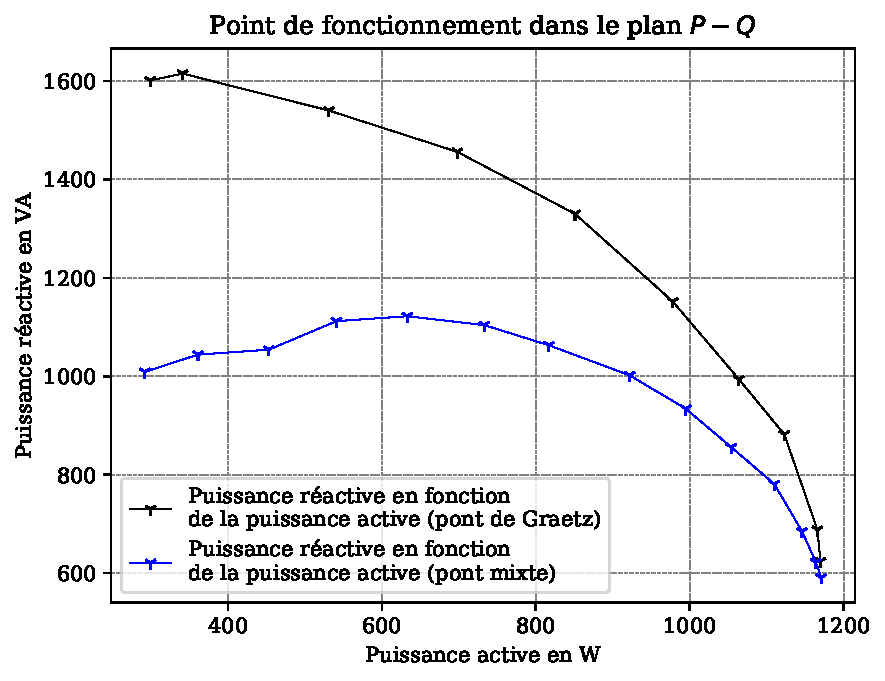
\includegraphics[width=0.8\linewidth]{cercle_PQ_complet}
    \caption{Diagramme $P-Q$ du pont mixte et du pont de Graetz}
    \label{fig:circle}
\end{figure}

La Figure~\ref{fig:circle} montre les diagrammes $P-Q$ du pont de Graetz et du pont mixte. On constate que pour les mêmes valeurs de puissances actives, les valeurs de puissances réactives sont inférieures. On a donc moins de pertes avec le pont mixte ce qui implique l'utilisation de moins de courant et donc de permet d'utiliser des câbles et de composants de calibres inférieurs. Cependant, le pont mixte ne peut pas fonctionner en onduleur.

\phantomsection
\section*{Conclusion}
\addcontentsline{toc}{section}{Conclusion}

Ce laboratoire nous a permis de déterminer (par mesure et de manière théorique) la caractéristique externe et l'angle d'empiètement ainsi que la caractéristique en terme de puissances actives et réactives de différents redresseurs à commutation naturelle (pont à point neutre, pont de Graetz et pont mixte).

En outre les différents avantages et inconvénients des différentes topologies ont été mis en avant (pertes, facteur de puissance, éventuelles économies sur la conception, conversion bidirectionnelle, etc.).\\

N.B. : Vous pouvez retrouvez le code utilisé pour générer les graphiques et le code de ce rapport sur GitHub : \url{https://github.com/2010019970909/power_electronics_reports}
\end{document}
